
\subsubsection{\stid{4.16} ALPINE} 


\paragraph{Overview} 

ECP ALPINE/{\zfp} will deliver in situ visualization and analysis infrastructure along with lossy compression for floating point arrays to ECP Applications.  

\textbf{ALPINE} developers come from the ParaView~\cite{alpine:Paraview1,alpine:Paraview2} and VisIt~\cite{alpine:VisIt} teams and ALPINE solutions will deliver in situ functionality in those tools, as well as through Ascent~\cite{alpine:Ascent}, a new in situ infrastructure framework that focuses on flyweight processing. 
%
ALPINE  focuses on four major activities: 
\begin{enumerate}
        \setlength{\itemsep}{1pt}
        \setlength{\parskip}{0pt}
        \setlength{\parsep}{0pt}
\item Deliver Exascale visualization and analysis algorithms that will be critical for ECP Applications as the dominant analysis paradigm shifts from post hoc (post-processing) to in situ (processing data in a code as it is generated). 
\item Deliver an Exascale-capable infrastructure for the development of in situ algorithms and deployment into existing applications, libraries, and tools. 
\item Engage with ECP Applications to integrate our algorithms and infrastructure into their software. 
\item Engage with ECP Software Technologies to integrate their Exascale software into our infrastructure. 
\end{enumerate}


\paragraph{Key  Challenges}

Many high performance simulation codes are using post hoc processing.  
Given Exascale I/O and storage constraints, in situ processing will be necessary. 
In situ data analysis and visualization selects, analyzes, reduces, and generates extracts from scientific simulation results during the simulation runs to overcome bandwidth and storage bottlenecks associated with writing out full simulation results to disk. 
The ALPINE team is addressing two problems related to Exascale processing --- (1) delivering infrastructure and (2) delivering performant in situ algorithms.
The challenge is that our existing infrastructure tools need to be made Exascale-ready in order to 
achieve performance within simulation codes' time budgets, support many-core architectures, scale to massive concurrency, and leverage deep memory hierarchies.
The challenge for in situ algorithms is to apply in situ processing effectively without a human being in the loop.
This means that we must have adaptive approaches to automate saving the correct visualizations and data extracts.


\paragraph{Solution Strategy}

A major strategy for our team is to leverage existing, successful software, ParaView and VisIt, including their  in situ libraries Catalyst~\cite{Catalyst} and LibSim~\cite{alpine:LibSim}, and then to integrate and augment them with ALPINE capabilities to address the challenges of Exascale. 
%
Both software projects represent long-term DOE investments, and they are the two dominant software packages for large-scale visualization and analysis within the DOE Office of Science (SC) and the DOE National Nuclear Security Agency (NNSA). 
These two products provide significant coverage of ECP Applications, and we can leverage their existing engagements to deliver ALPINE's algorithms and infrastructure. 
%Our development strategy consists of placing all new algorithms developed in a single code repository, and deploying this code in both
%ParaView and VisIt.
%
We are also developing an additional  in situ framework, Ascent.  Ascent is a ``flyweight'' solution, meaning that it is focused on a streamlined API, minimal memory footprint, and small binary size.
Our solution strategy is two-fold, in response to our two major challenges: infrastructure and algorithms.

For infrastructure, we have developed a layer on top of the VTK-m library for ALPINE algorithms.
This layer is where all ALPINE algorithms will be implemented, and it is deployed in ParaView/Catalyst, VisIt, and Ascent.
Thus all development effort by ALPINE will be available in all of our tools.
Further, by leveraging VTK-m, we will be addressing issues with many-core architectures.  
Figure~\ref{fig:alpine_infrastructure} illustrates our software strategy.

\begin{figure}[htb]
	\centering
	\includegraphics[width=3in]{projects/2.3.4-DataViz/2.3.4.16-ALPINE-ZFP/alpine_infrastructure.png}
	\caption{\label{fig:alpine_infrastructure}ALPINE's strategy for delivering and developing software.  We are making use of existing software (ParaView, VisIt), but making sure all new development is shared in all of our tools.  The dotted lines represent ongoing work, specifically that the Ascent API will work with ParaView and VisIt.}
\end{figure}

ALPINE is developing a suite of in situ  algorithms designed to address I/O and data output constraints.   These algorithms include:.  
\begin{description}  
	\setlength{\itemsep}{1pt}
    \setlength{\parskip}{0pt}
    \setlength{\parsep}{0pt}
	\item [Topological analysis] can be used to detect features in the data and adaptively steer visualizations with no human in the loop.  For example, contour trees can identify the most significant isosurfaces in complex simulations and then the resulting visualizations can use these isosurfaces~\cite{alpine:Carr:TVCG19}.
	\item [Adaptive sampling]  can be used to guide visualizations and extracts to the most important parts of the simulation, significantly reducing I/O.  Figure~\ref{fig:alpine-sampling-example} shows an adaptive sampling technique based on importance to preserve  features in the data~\cite{alpine:Biswas:ISAV18,alpine:Dutta:Entropy19,alpine:Liu:SC19poster}.
	\item [Statistical feature detection] models data using distribution-based approaches and statistical similarity measures to identify and isolate features of interest~\cite{alpine:Dutta:PVIS17,alpine:Dutta:VIS15}. Significant data reduction is possible by only saving the statistical representations of the data.  Figure~\ref{fig:alpine-statistical-feature} illustrates the use of the statistical feature detection approach to identifying bubbles in situ in an MFiX-Exa simulation.  
	\item [Task-based feature extraction] uses segmented merge trees to encode a wide range of threshold based features.  An embedded domain specific language (EDSL) can describe algorithms using a  task graph abstraction~\cite{alpine:Landge:SC14,alpine:Petruzza:IPDPS18} and execute it using different runtimes (e.g., MPI, Charm++, Legion).
	\item [Optimal Viewpoint] Optimal viewpoint metrics are used to automate visualization decisions while running in situ.  This initial development will choose the best camera placement for a scene.  
	\item [Lagrangian analysis] of vector flow allows more efficient and complete tracking of flow.  It can save vector field data with higher accuracy and less storage than the traditional approaches~\cite{alpine:Sane:EGPGV18,alpine:Sane:EGPGV19,alpine:Binyahib:LDAV19}.
	\item [Moments-based pattern detection] can be used to find rotation-invariant patterns~\cite{alpine:Bujack:WSCG17,alpine:Yang:PR17,alpine:Wang:TopoVis17}. 
\end{description}

\begin{figure*}[htb]
	\begin{center}
		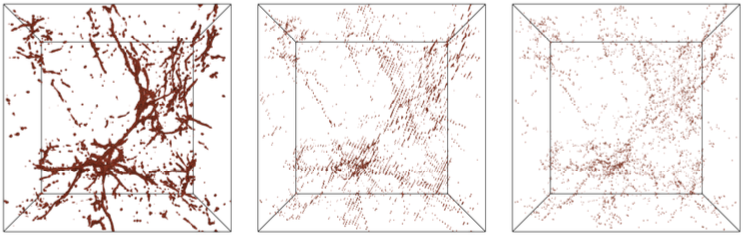
\includegraphics[width=0.65\textwidth]{projects/2.3.4-DataViz/2.3.4.16-ALPINE-ZFP/alpine_nyxSamplingExample.png}
		\caption{Point rendering results from Nyx simulation using (left to right):  ALPINE adaptive sampling  (sampling ratio 0.5\%); regular sampling  (sampling ratio 1.5\%); random sampling  (sampling ratio 0.5\%).}
		\label{fig:alpine-sampling-example}
	\end{center}
\end{figure*}

\paragraph{Recent Progress}

During this past year, ALPINE has made considerable progress in core functionality in infrastructure and algorithms, and in creating a robust software stack to meet exascale data and viz needs.  ALPINE rolled out continuous integration for ParaView and Ascent, improving the Spack build systems.  Documentation has been rolled out for algorithms (https://alpine-dav.readthedocs.io/en/latest/).  ALPINE team members have ported ParaView and VisIt to Summit and built Ascent on Iris.  

\textbf{UPDATE}
In recent milestones, we integrated the team’s mature and emerging algorithms into the ALPINE infrastructure (STDA04-32, STDA04-41, STDA04-43) and demonstrated early in situ implementations in ECP codes (STDA04-33) with demonstrations of parallel distributed versions for each mature algorithm (STDA04-37).  Emerging algorithms have been prototyped with ECP applications.  
In a final FY19 milestone for these algorithms, we demonstrated end-to-end integration pipelines with ECP Applications and ALPINE infrastructure for other in situ algorithms (STDA04-38):

\begin{itemize}  
	\setlength{\itemsep}{1pt}
	\setlength{\parskip}{0pt}
	\setlength{\parsep}{0pt}
	\item ExaSky:Nyx was integrated with Ascent, running adaptive sampling and outputting a Cinema database; demonstrated on Summit with ALPINE codes on the GPUs and Nyx on the CPUs. 
	\item EQSIM:SW4 was integrated with Ascent, running the Lagrangian algorithm; demonstrated on Summit GPUs.  
	\item WarpX was integrated with Ascent and accessed the Moments-based pattern detection algorithm through ParaView; demonstrated on Summit CPUs.
	\item PeleC was integrated with Ascent, running adaptive sampling; demonstrated on Summit CPUs.
\end{itemize}


\begin{figure*}[htb]
	\begin{center}
		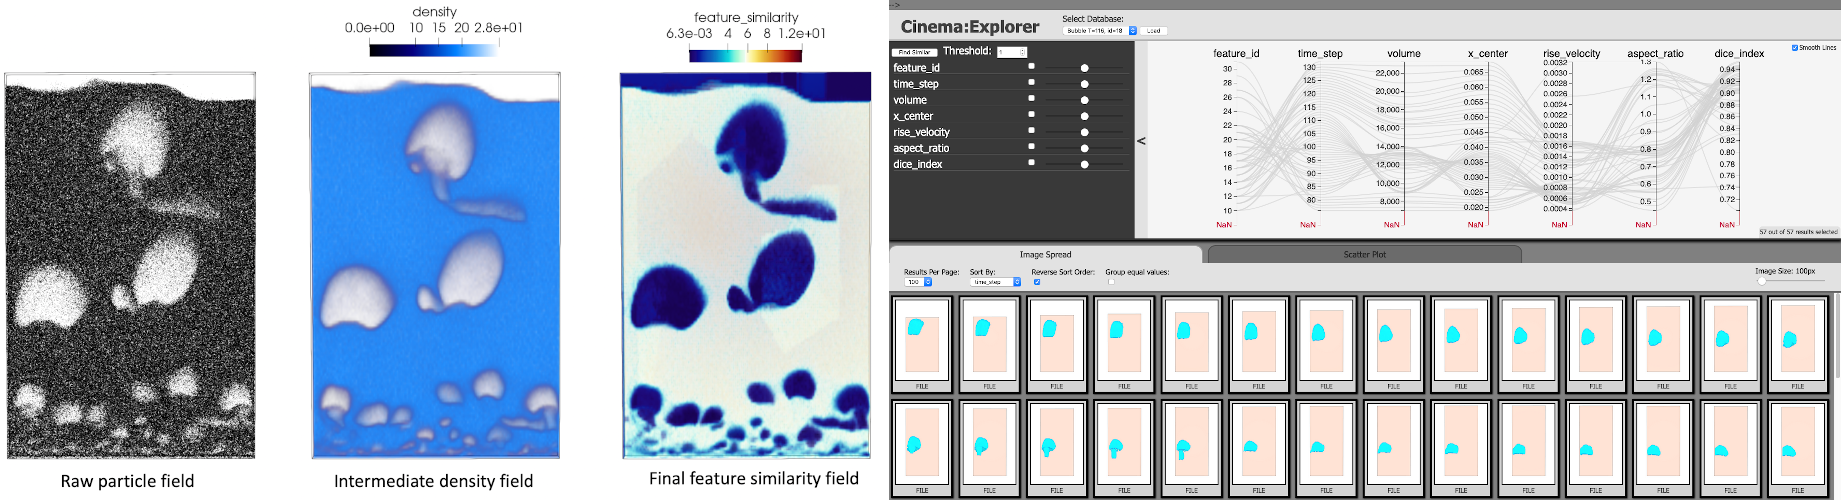
\includegraphics[width=0.95\textwidth]{projects/2.3.4-DataViz/2.3.4.16-ALPINE-ZFP/alpine-cinema-mfixexa-workflow.png}
		\caption{The ALPINE statistical feature detection algorithm is used to identify bubbles in situ in an MFiX-Exa fluidized bed simulation.  The raw particle data is converted to a particle density field.  A threshold is applied to the density field to create a feature similarity field, separating the bubbles from uninteresting regions.  Saving only the statistical representation allows greater temporal resolution while significantly reducing output data size.  A preliminary study shows a factor of 300 reduction in data size compared to the raw particle fields. The statistical bubble representation becomes the input to a post hoc Cinema-based workflow that can be used to track bubbles and explore bubble dynamics. }
		\label{fig:alpine-statistical-feature}
	\end{center}
\end{figure*}

\paragraph{Next Steps}

Plans for FY21-23 will continue the focus of integration and delivery to ECP applications. The emphasis in 2020 and 2021 will be porting the team’s software products to Frontier and Aurora, doing initial performance studies relevant to ECP applications. The team will also focus on outreach and prototyping integrations with ECP application codes in order to facilitate full integration in later years.

